% !TeX spellcheck = en_US
% !TEX root = ../thesis-example.tex
%
\chapter{Outlook}

Motion capturing solution usually support a live preview of the actors motion 
inside a 3D environment - integrating an actor into a virtual world is not only 
in interest of VR developers, but motion video productions, too. Mixed Reality 
is an increasingly important topic for VR experiences. The number of MR-enabled 
or MR-captured software is increasing, likely due to the natural way of 
producing video material and easily understandable usage context of that 
software. Since stereo-rendering already requires the GPU to do multiple 
context switches per frame, future hardware will probably improve on that 
matter, enabling better performance for a complex Mixed Reality pipelines.

\section{Rendering Setup Variations}

There are a few approaches that work similarly, but differ with respect to 
complexity, their capabilities and hardware requirements. They have been 
already explored by producing companies and are covered here for completeness.

\subsection{Single Camera - 3D Plane in Space}

A novel approach is rendering the camera image onto a 2D plane positioned 
inside the 3D scene. This gives high control over projection parameters inside 
the engine without a running software and has good visual feedback for artists. 
All additional steps previously discussed are invalid, since this render can 
take full advantage of all runtime rendering parameters - which in turn means 
for lower render overhead and better graphical performance. It fails however on 
delay mitigation, which makes time drift between engine and camera visible, 
thus only usable with low latency video capturing devices. (Figure 
\ref{fig:alt-render:single-camera} for reference)

\begin{figure}[htb]
	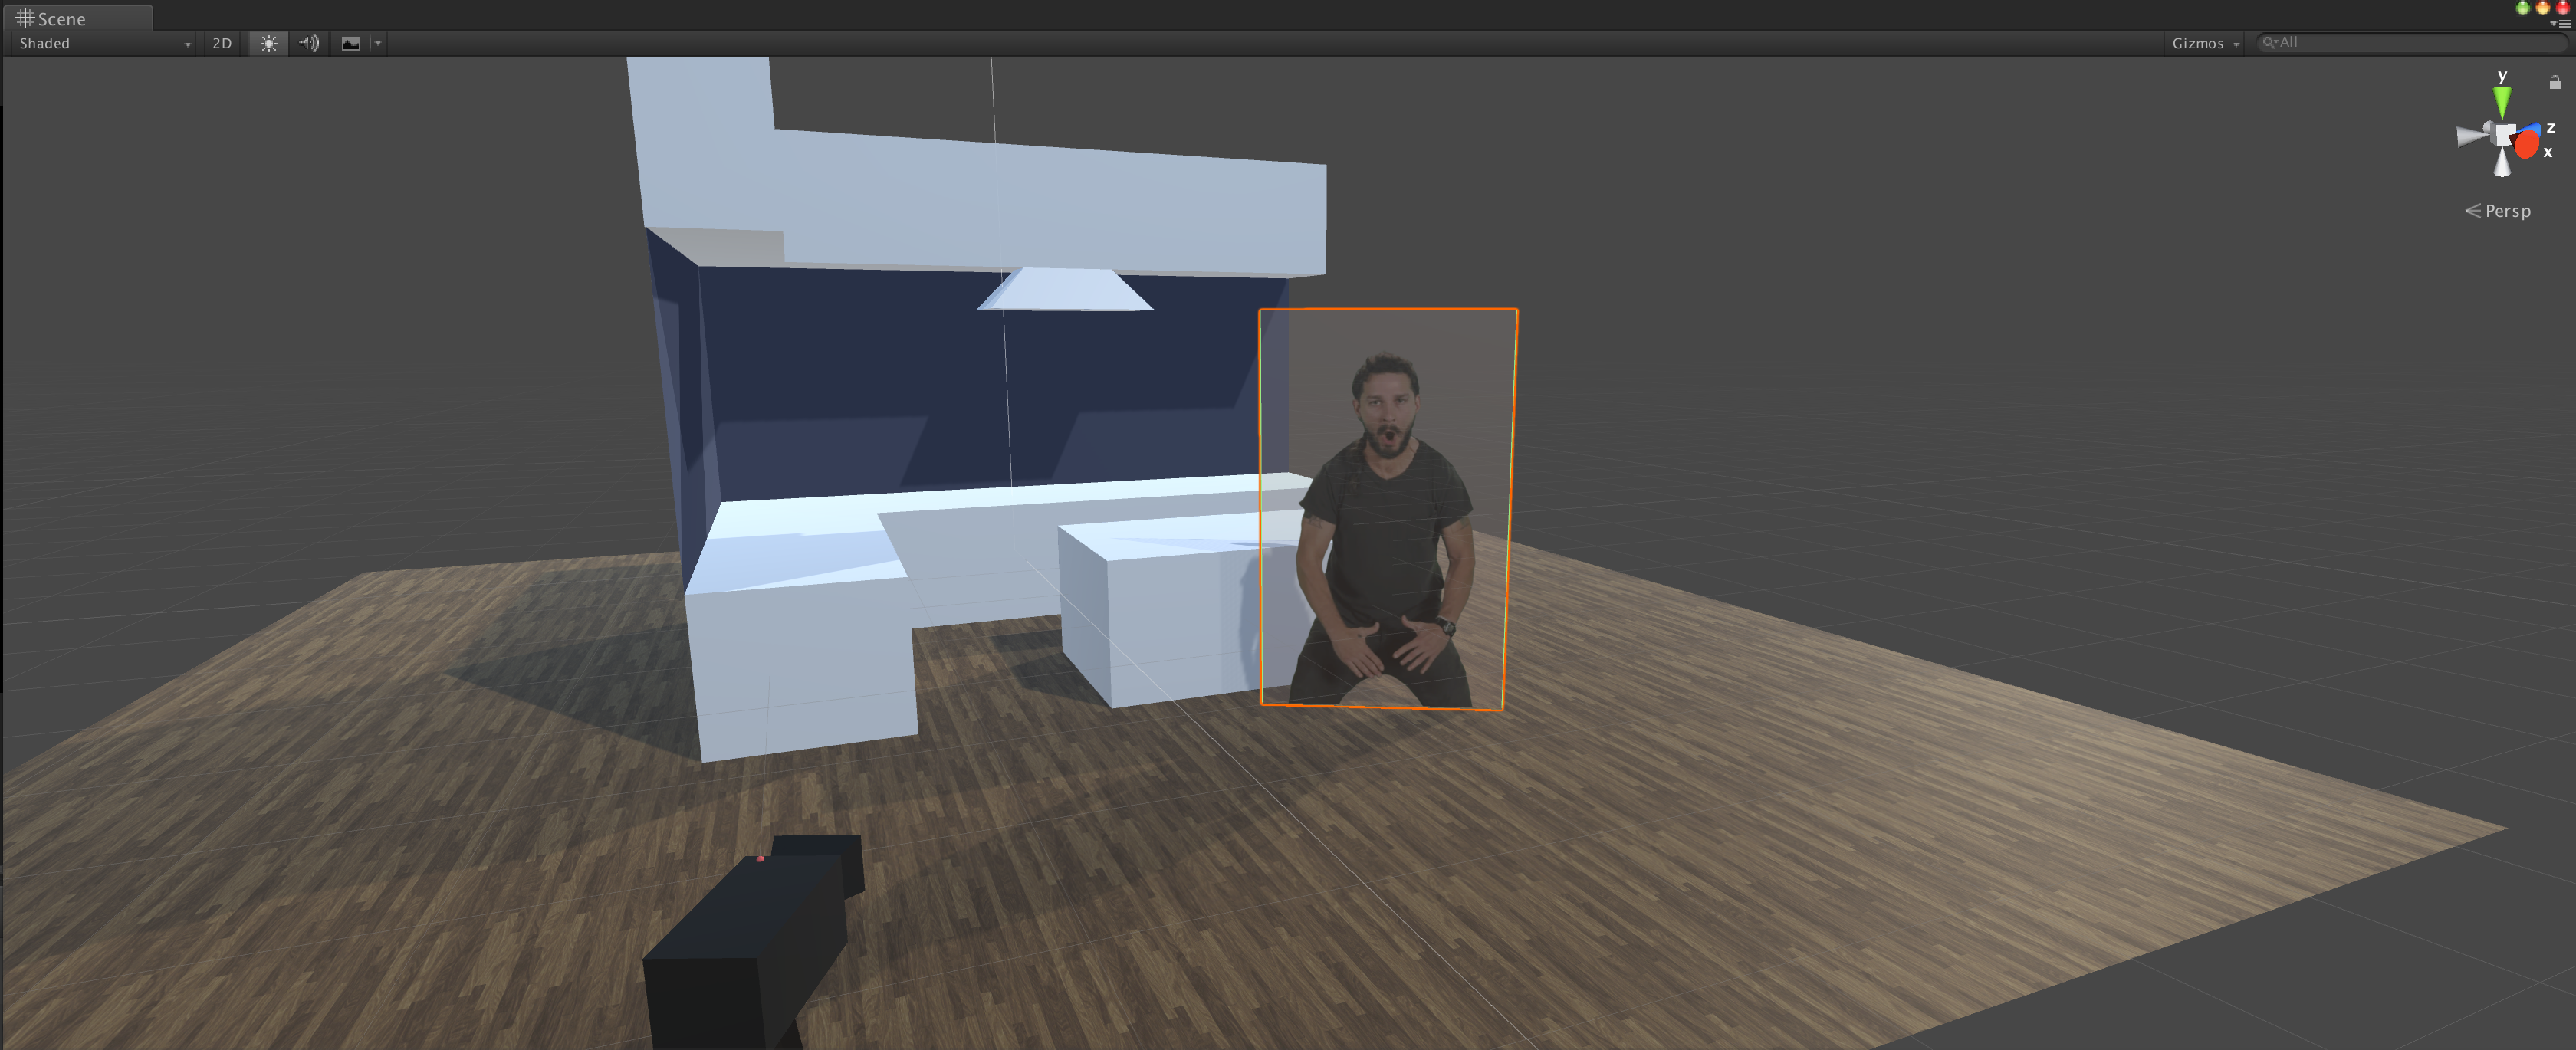
\includegraphics[width=\textwidth]{gfx/eval/plane-scene.png}
	\caption{Demonstrative scene with a plane at camera's rendering position}
	\label{fig:alt-render:single-camera}
\end{figure}

\subsection{Deferred Shading Path}

Similarly to the single camera approach, a deferred shader could be used, in 
which the plane is projected and texturized after the scene has rendered and 
the graphics buffer is still present - this way the total time taken for 
rendering can be calculated and the chroma keying step can be chosen for a 
faster variant if needed. This gives generally better control and could yield 
higher performance, since all projected fragments have an assigned depth - the 
camera image only has to be calculated where the actor's depth is smaller than 
the scenery's depth. This method is also lacking a way of adjusting for time 
drift. Additionally, calculating lightning is relatively expensive, due to the 
reprojection of lighting parameters inside the graphics buffer. A snapshot of 
this buffer cannot be stored - which is a limitation of Unity's render pipeline 
- and is lost after the rendering loop is completed.

\subsection{Composition Workstation (4 patch)}

Lastly, for full video production setups another rendering approach has been 
suggested, which has been used for the initial promo material for the HTC 
Vive\cite{valve:vive-trailer:2016}. It includes rendering a 4K video signal, 
outputting it to a composition PC which then takes care about managing time 
drift and video input from the camera.
\newline
The general concept involves a production of four 1920x1080 video signals of 
the virtual environment:
\begin{my_list}
	\item Background
	\item Foreground with blue matte
	\item Composite image
	\item First person view
\end{my_list}

\begin{figure}[htb]
	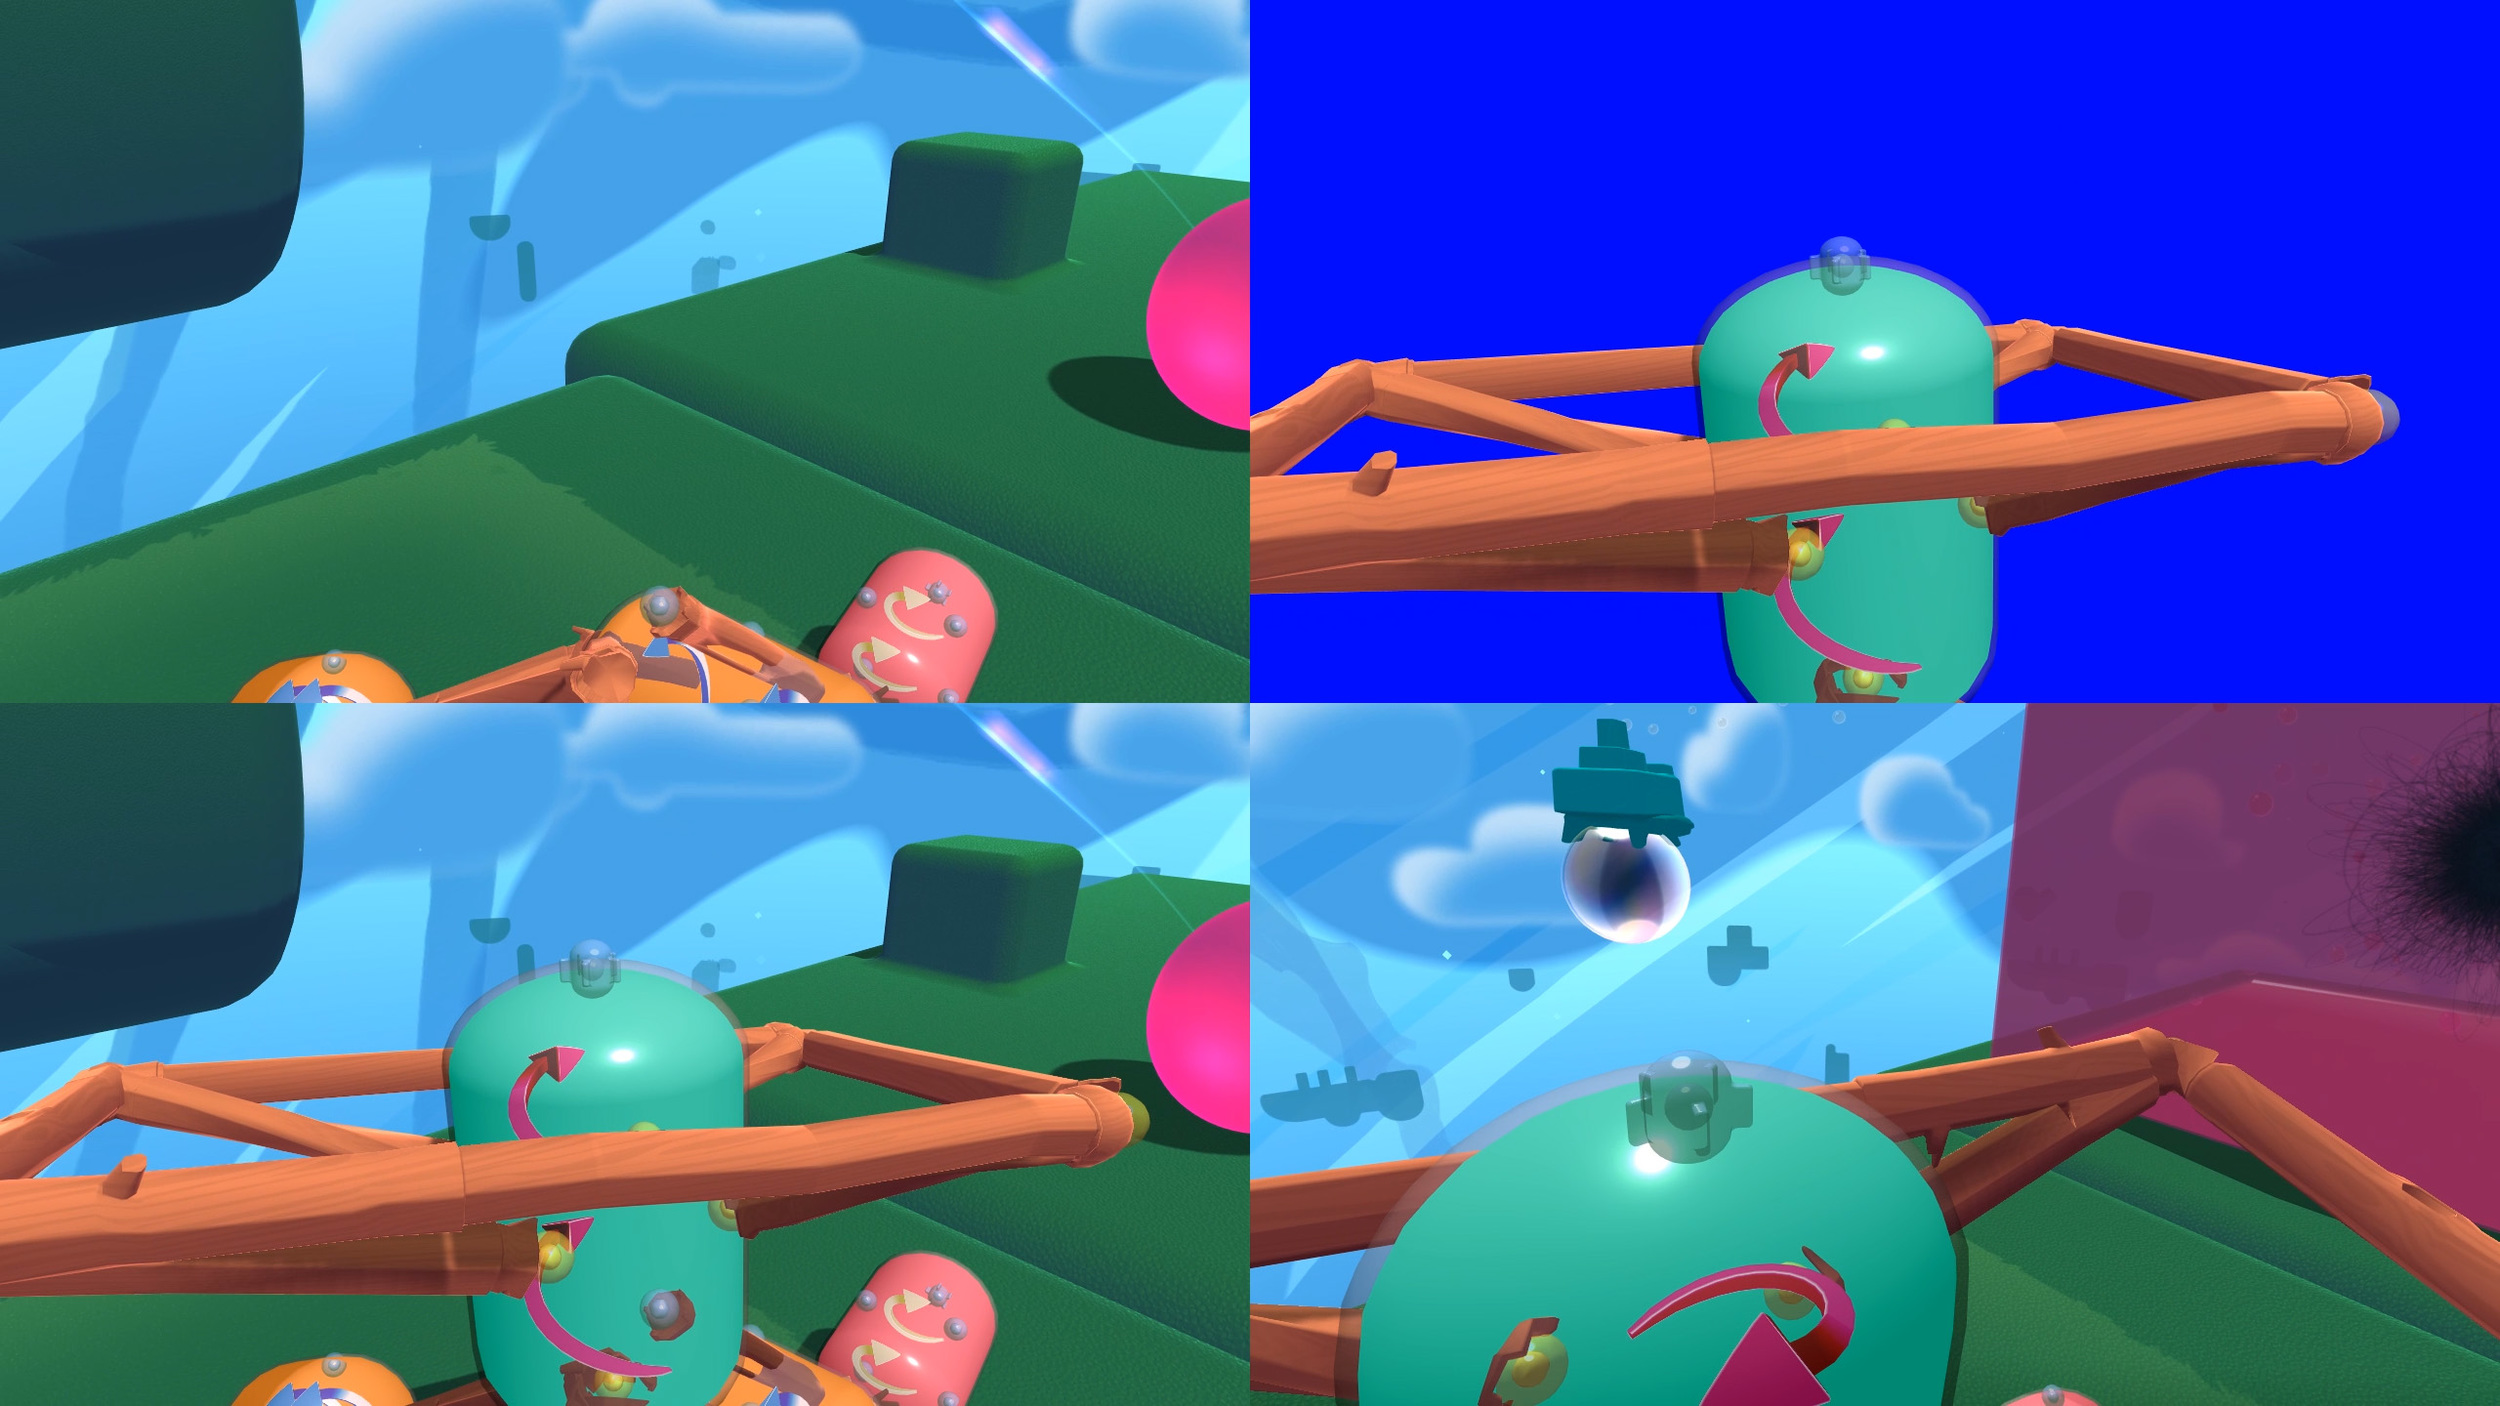
\includegraphics[width=\textwidth]{_external/media/4patch.jpg}
	\caption{4 Patch output for post / second station 
		production\cite{gartner:mixed-reality:2017}.}
	\label{fig:alt-render:4patch}
\end{figure}

Due to the system separation it is now possible to use green screen hardware 
compositors which have a visually higher quality in pulling the green 
background matte and then compositing it similarly into a mixed reality image. 
While this lifts some rendering overhead from the host PC, it fails in 
recreating a lightning environment for the VR actor and relies on two systems. 
While engine programming complexity decreases, operational setup complexity 
increases.

\section{Rendering Operational Variations}

This setup can handle another operational context by leaving out 
background-sorting and only rendering a virtual "front", by which a high 
quality augmented camera system can be achieved. Since time drift between 
camera and engine is already handled, it is possible to render an augmented 
image. Since depth information is lost, it is not possible to handle 
obstructions - for example by an interacting user that is standing in front of 
the augmented object. However, with some composition and choreography, AR 
footage can be showed and captured in live production for further use. A 
reference plane has to be used, either by a Vive Tracker\footnote{like a 
controller} or with feature markers.
\newline
This thesis assumes that the motion video feed is calibrated for a D65 white 
and augmented reality scenarios usually do not take real-world lightning into 
account, it would give a good natural and high quality look into augmented 
reality use cases.

\section{Multi User Augmented Reality}

While working with this setup another possible use-case showed up: On June 2017 
Apple presented their native Augmented Reality kit integrated in their consumer 
devices. Thus a similar system could be used to send all tracking parameters 
from the HTC Vive headset to these devices and have a calibrated north-wall 
with additional feature markers. This would potentially allow to have an 
augmented reality view around the actors world with a fast approximated actor 
position. It could then be possible for multiple users to use these devices as 
window into the virtual reality experience without a green screen at all.